\documentclass[border=12pt]{standalone}
\usepackage[T1]{fontenc}
\usepackage{tikz}
\usepackage{amsmath,amssymb}
\usepackage{xcolor}

\usetikzlibrary{
  shapes.geometric,
  arrows.meta,
  positioning,
  fit,
  backgrounds,
  calc,
  decorations.pathreplacing,
  shadows.blur
}

% ── Colour palette ──────────────────────────────────────────────────
\definecolor{rosettaCol}{HTML}{E8D5B7}      % warm beige
\definecolor{cgCol}{HTML}{B8D4E3}           % soft blue
\definecolor{membraneCol}{HTML}{C5E0B4}     % soft green
\definecolor{cgEqCol}{HTML}{D5C4E0}         % soft purple
\definecolor{backmapCol}{HTML}{F4B183}      % soft orange
\definecolor{aaEqCol}{HTML}{FFD966}         % gold
\definecolor{prodCol}{HTML}{FF7C80}         % soft red
\definecolor{analysisCol}{HTML}{A9D18E}     % green
\definecolor{arrowCol}{HTML}{404040}        % dark grey
\definecolor{boxBorder}{HTML}{333333}       % near-black
\definecolor{paramBg}{HTML}{F7F7F7}         % very light grey
\definecolor{hwCol}{HTML}{D9E2F3}           % light steel blue

% ── Styles ──────────────────────────────────────────────────────────
\tikzset{
  mainbox/.style={
    draw=boxBorder, line width=1pt,
    rounded corners=6pt,
    minimum width=13.5cm, minimum height=1.6cm,
    text width=13cm, align=center,
    font=\sffamily\bfseries\large,
    blur shadow={shadow blur steps=4, shadow xshift=0.8pt, shadow yshift=-0.8pt}
  },
  parambox/.style={
    draw=boxBorder!60, line width=0.4pt,
    rounded corners=3pt,
    fill=paramBg,
    text width=12.5cm, align=left,
    font=\sffamily\scriptsize,
    inner sep=5pt
  },
  substage/.style={
    draw=boxBorder!50, line width=0.5pt,
    rounded corners=3pt,
    minimum width=2.6cm, minimum height=0.7cm,
    text width=2.4cm, align=center,
    font=\sffamily\scriptsize\bfseries,
    fill=#1!30
  },
  stagenum/.style={
    circle, draw=boxBorder, line width=0.8pt,
    minimum size=7mm,
    font=\sffamily\bfseries\small,
    fill=white
  },
  thickarrow/.style={
    -Stealth, line width=1.5pt, color=arrowCol
  },
  branchArrow/.style={
    -Stealth, line width=1pt, color=arrowCol, dashed
  },
  groupbox/.style={
    draw=#1!80!black, line width=1.2pt,
    rounded corners=8pt,
    fill=#1!8,
    inner sep=8pt
  },
  annot/.style={
    font=\sffamily\tiny\itshape, text=black!70
  },
  sidelabel/.style={
    font=\sffamily\scriptsize, text=black!60, rotate=90, anchor=south
  },
  eqtable/.style={
    draw=boxBorder!40, line width=0.3pt,
    rounded corners=2pt,
    fill=#1!15,
    text width=1.8cm, minimum height=0.55cm,
    align=center,
    font=\sffamily\tiny
  }
}

\begin{document}
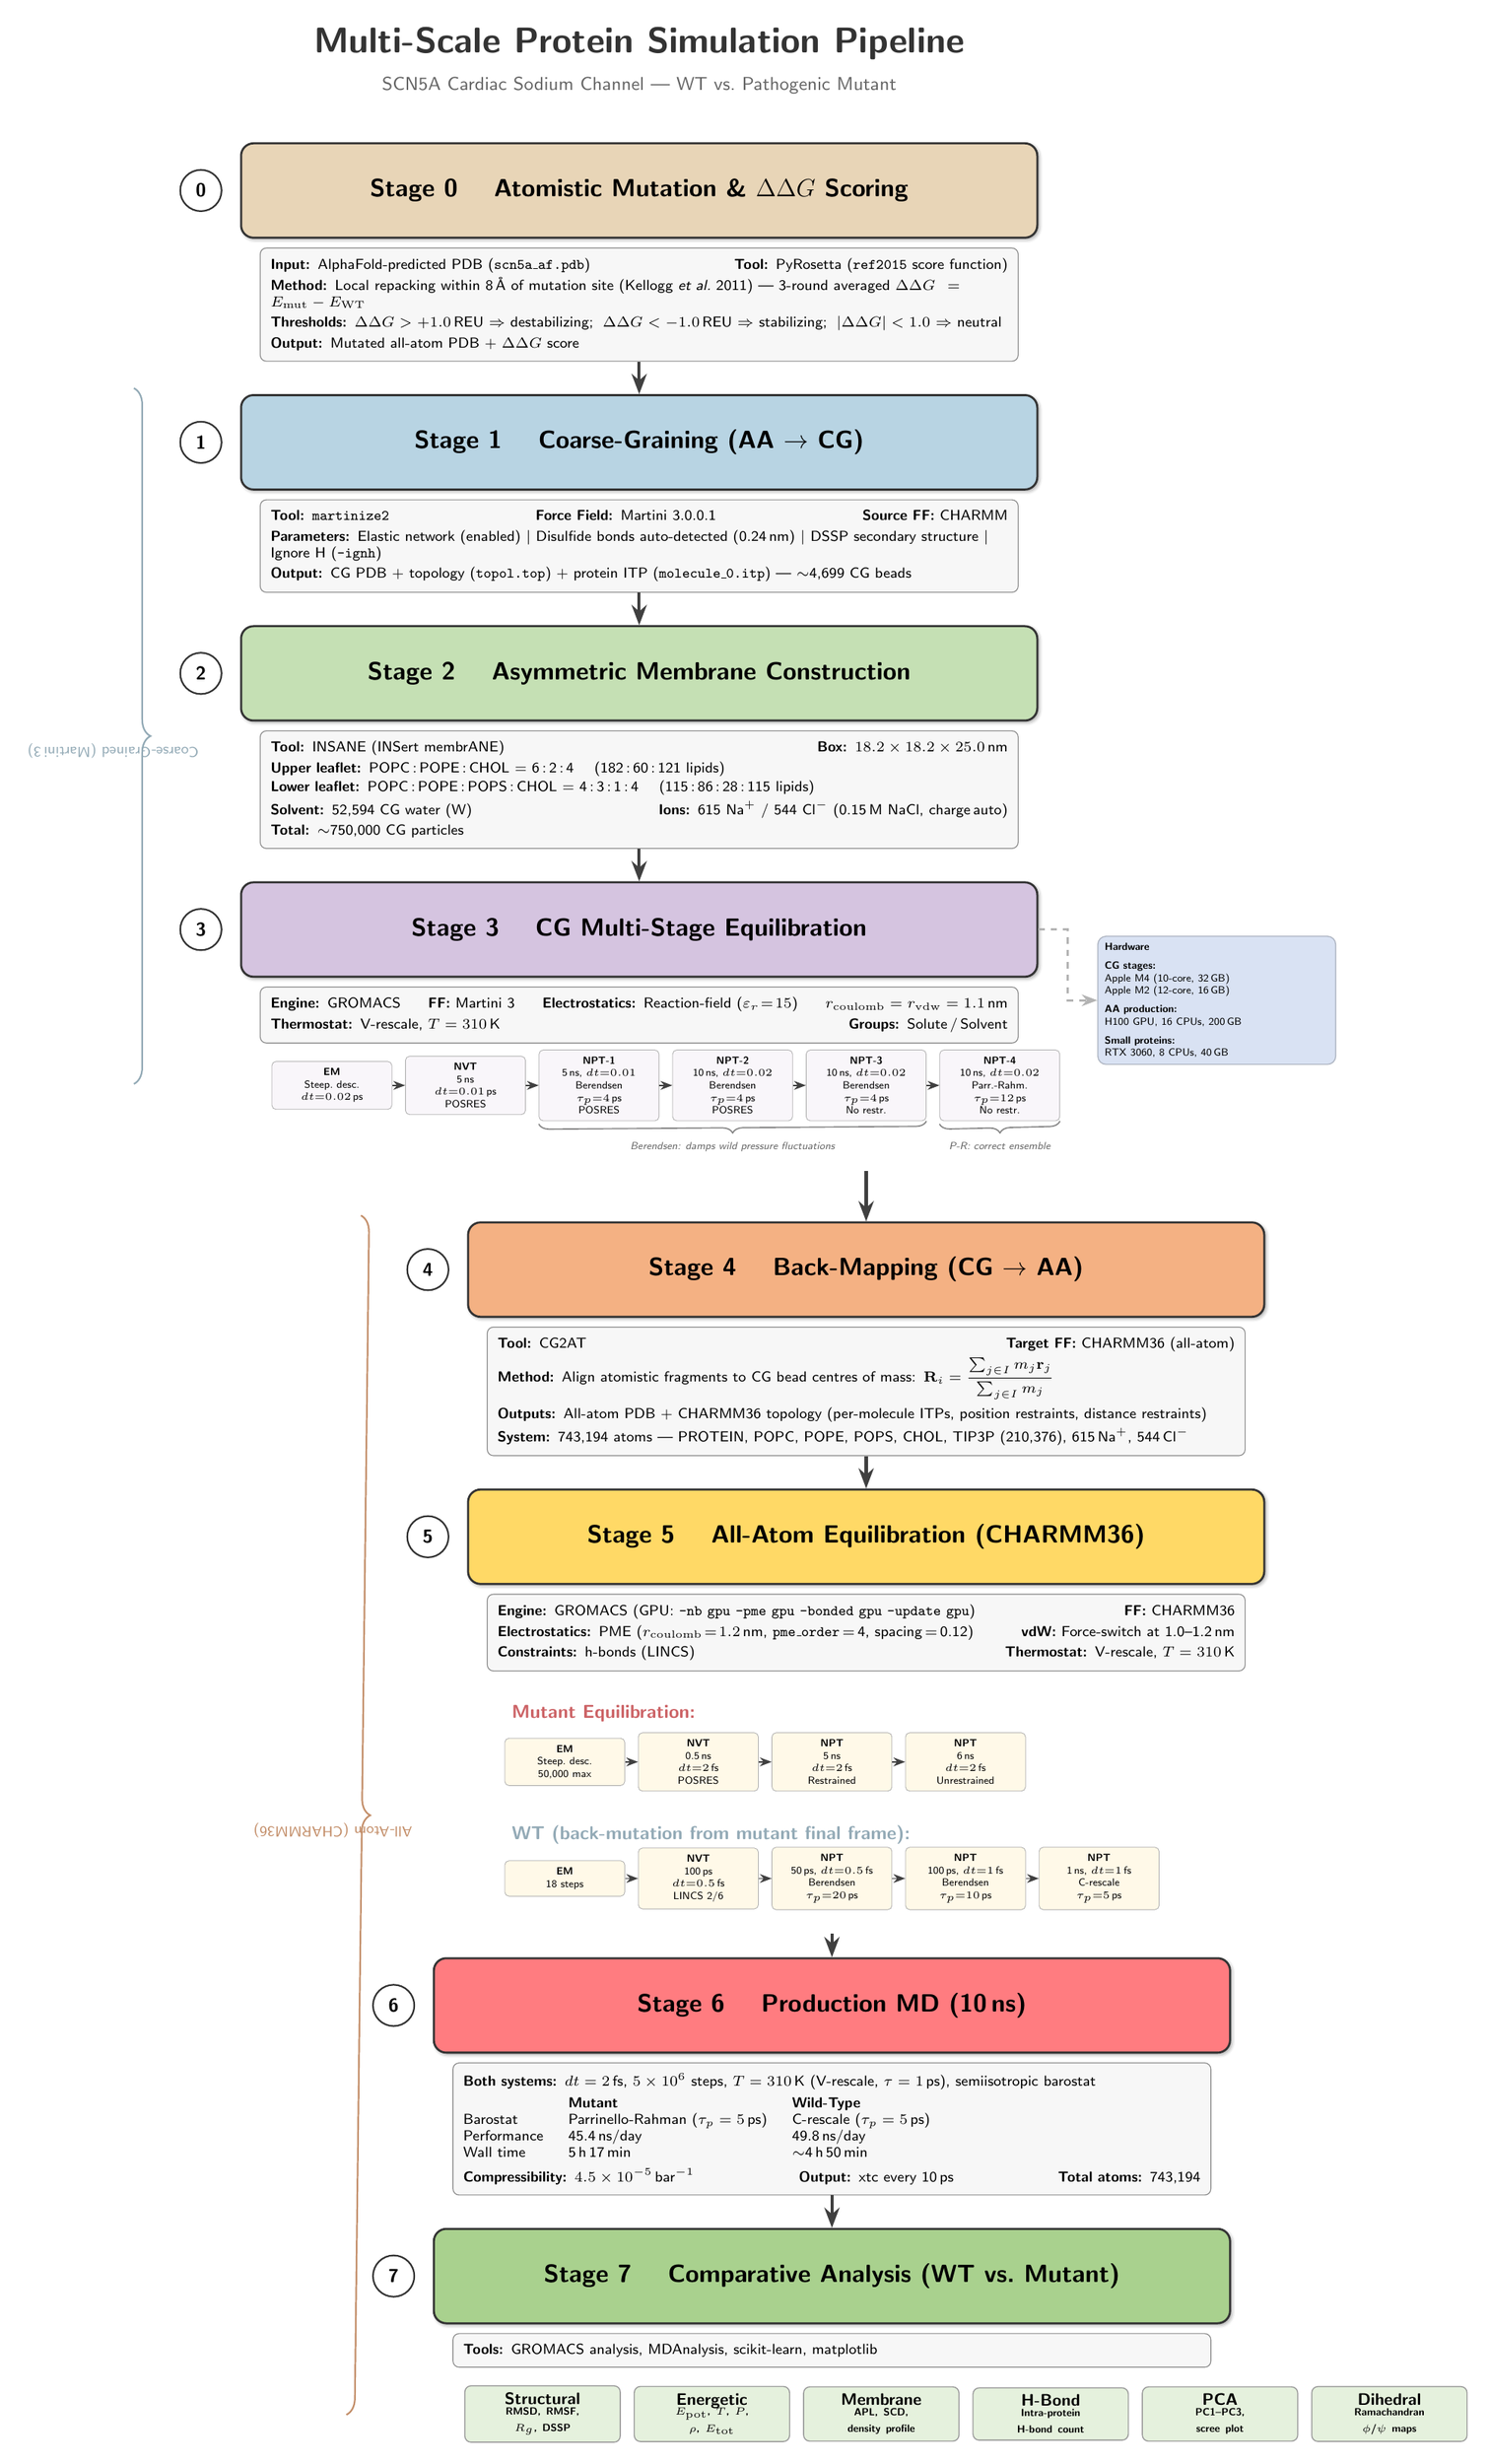
\begin{tikzpicture}[node distance=0.55cm]

% ══════════════════════════════════════════════════════════════════════
%  TITLE
% ══════════════════════════════════════════════════════════════════════
\node[font=\sffamily\bfseries\LARGE, text=boxBorder] (title)
  {Multi-Scale Protein Simulation Pipeline};
\node[below=0.05cm of title, font=\sffamily\small, text=black!60]
  (subtitle) {SCN5A Cardiac Sodium Channel --- WT vs.\ Pathogenic Mutant};

% ══════════════════════════════════════════════════════════════════════
%  STAGE 0 — Input / Rosetta Mutation
% ══════════════════════════════════════════════════════════════════════
\node[mainbox, fill=rosettaCol, below=0.7cm of subtitle] (S0)
  {\textsc{Stage 0} \quad Atomistic Mutation \& $\Delta\Delta G$ Scoring};
\node[stagenum, left=0.3cm of S0.west] {0};

\node[parambox, below=0.15cm of S0.south, anchor=north] (S0p) {%
  \textbf{Input:} AlphaFold-predicted PDB (\texttt{scn5a\_af.pdb}) \hfill
  \textbf{Tool:} PyRosetta (\texttt{ref2015} score function)\\[2pt]
  \textbf{Method:} Local repacking within 8\,\AA\ of mutation site
  (Kellogg \emph{et al.}\ 2011) --- 3-round averaged
  $\Delta\Delta G = E_{\mathrm{mut}} - E_{\mathrm{WT}}$\\[2pt]
  \textbf{Thresholds:}
  $\Delta\Delta G > +1.0$\,REU $\Rightarrow$ destabilizing;\;
  $\Delta\Delta G < -1.0$\,REU $\Rightarrow$ stabilizing;\;
  $|\Delta\Delta G| < 1.0$ $\Rightarrow$ neutral\\[2pt]
  \textbf{Output:} Mutated all-atom PDB + $\Delta\Delta G$ score
};

% ══════════════════════════════════════════════════════════════════════
%  STAGE 1 — Martinize2
% ══════════════════════════════════════════════════════════════════════
\node[mainbox, fill=cgCol, below=0.55cm of S0p.south, anchor=north] (S1)
  {\textsc{Stage 1} \quad Coarse-Graining (AA $\rightarrow$ CG)};
\node[stagenum, left=0.3cm of S1.west] {1};

\node[parambox, below=0.15cm of S1.south, anchor=north] (S1p) {%
  \textbf{Tool:} \texttt{martinize2} \hfill
  \textbf{Force Field:} Martini 3.0.0.1 \hfill
  \textbf{Source FF:} CHARMM\\[2pt]
  \textbf{Parameters:}
  Elastic network (enabled) \textbar\
  Disulfide bonds auto-detected (0.24\,nm) \textbar\
  DSSP secondary structure \textbar\
  Ignore H (\texttt{-ignh})\\[2pt]
  \textbf{Output:} CG PDB + topology (\texttt{topol.top}) +
  protein ITP (\texttt{molecule\_0.itp}) --- $\sim$4{,}699 CG beads
};

% arrow
\draw[thickarrow] (S0p.south) -- (S1.north);

% ══════════════════════════════════════════════════════════════════════
%  STAGE 2 — INSANE membrane
% ══════════════════════════════════════════════════════════════════════
\node[mainbox, fill=membraneCol, below=0.55cm of S1p.south, anchor=north] (S2)
  {\textsc{Stage 2} \quad Asymmetric Membrane Construction};
\node[stagenum, left=0.3cm of S2.west] {2};

\node[parambox, below=0.15cm of S2.south, anchor=north] (S2p) {%
  \textbf{Tool:} INSANE (INSert membrANE) \hfill
  \textbf{Box:} $18.2 \times 18.2 \times 25.0$\,nm\\[2pt]
  \textbf{Upper leaflet:} POPC\,:\,POPE\,:\,CHOL = 6\,:\,2\,:\,4
  \quad (182\,:\,60\,:\,121 lipids)\\[1pt]
  \textbf{Lower leaflet:} POPC\,:\,POPE\,:\,POPS\,:\,CHOL = 4\,:\,3\,:\,1\,:\,4
  \quad (115\,:\,86\,:\,28\,:\,115 lipids)\\[2pt]
  \textbf{Solvent:} 52{,}594 CG water (W) \hfill
  \textbf{Ions:} 615 Na$^{+}$ / 544 Cl$^{-}$ (0.15\,M NaCl, charge\,auto)\\[2pt]
  \textbf{Total:} $\sim$750{,}000 CG particles
};

\draw[thickarrow] (S1p.south) -- (S2.north);

% ══════════════════════════════════════════════════════════════════════
%  STAGE 3 — CG Equilibration
% ══════════════════════════════════════════════════════════════════════
\node[mainbox, fill=cgEqCol, below=0.55cm of S2p.south, anchor=north] (S3)
  {\textsc{Stage 3} \quad CG Multi-Stage Equilibration};
\node[stagenum, left=0.3cm of S3.west] {3};

\node[parambox, below=0.15cm of S3.south, anchor=north] (S3p) {%
  \textbf{Engine:} GROMACS \hfill
  \textbf{FF:} Martini 3 \hfill
  \textbf{Electrostatics:} Reaction-field ($\varepsilon_r\!=\!15$) \hfill
  $r_{\mathrm{coulomb}} = r_{\mathrm{vdw}} = 1.1$\,nm\\[2pt]
  \textbf{Thermostat:} V-rescale, $T = 310$\,K \hfill
  \textbf{Groups:} Solute\,/\,Solvent
};

% sub-stage row
\node[eqtable=cgEqCol, below=0.3cm of S3p.south west, anchor=north west,
      xshift=0.2cm] (eq1)
  {\textbf{EM}\\Steep.\ desc.\\$dt{=}0.02$\,ps};

\node[eqtable=cgEqCol, right=0.22cm of eq1] (eq2)
  {\textbf{NVT}\\5\,ns\\$dt{=}0.01$\,ps\\POSRES};

\node[eqtable=cgEqCol, right=0.22cm of eq2] (eq3)
  {\textbf{NPT-1}\\5\,ns, $dt{=}0.01$\\Berendsen\\$\tau_p{=}4$\,ps\\POSRES};

\node[eqtable=cgEqCol, right=0.22cm of eq3] (eq4)
  {\textbf{NPT-2}\\10\,ns, $dt{=}0.02$\\Berendsen\\$\tau_p{=}4$\,ps\\POSRES};

\node[eqtable=cgEqCol, right=0.22cm of eq4] (eq5)
  {\textbf{NPT-3}\\10\,ns, $dt{=}0.02$\\Berendsen\\$\tau_p{=}4$\,ps\\No restr.};

\node[eqtable=cgEqCol, right=0.22cm of eq5] (eq6)
  {\textbf{NPT-4}\\10\,ns, $dt{=}0.02$\\Parr.-Rahm.\\$\tau_p{=}12$\,ps\\No restr.};

% arrows between sub-stages
\foreach \a/\b in {eq1/eq2, eq2/eq3, eq3/eq4, eq4/eq5, eq5/eq6}{
  \draw[-Stealth, line width=0.6pt, arrowCol] (\a.east) -- (\b.west);
}

% Brace annotation
\draw[decorate, decoration={brace, amplitude=5pt, mirror},
      line width=0.6pt, boxBorder!60]
  (eq3.south west) ++(0,-0.05) -- (eq5.south east |- eq3.south west)
  node[midway, below=6pt, font=\sffamily\tiny\itshape, text=black!60]
  {Berendsen: damps wild pressure fluctuations};

\draw[decorate, decoration={brace, amplitude=5pt, mirror},
      line width=0.6pt, boxBorder!60]
  (eq6.south west) ++(0,-0.05) -- (eq6.south east)
  node[midway, below=6pt, font=\sffamily\tiny\itshape, text=black!60]
  {P-R: correct ensemble};

\draw[thickarrow] (S2p.south) -- (S3.north);

% ══════════════════════════════════════════════════════════════════════
%  STAGE 4 — CG2AT Back-mapping
% ══════════════════════════════════════════════════════════════════════
\coordinate (belowEq) at ($(eq5.south)+(0,-0.85)$);

\node[mainbox, fill=backmapCol, below=0.85cm of belowEq, anchor=north] (S4)
  {\textsc{Stage 4} \quad Back-Mapping (CG $\rightarrow$ AA)};
\node[stagenum, left=0.3cm of S4.west] {4};

\node[parambox, below=0.15cm of S4.south, anchor=north] (S4p) {%
  \textbf{Tool:} CG2AT \hfill
  \textbf{Target FF:} CHARMM36 (all-atom)\\[2pt]
  \textbf{Method:} Align atomistic fragments to CG bead centres of mass:
  $\displaystyle\mathbf{R}_i =
    \frac{\sum_{j\in I} m_j \mathbf{r}_j}{\sum_{j\in I} m_j}$\\[3pt]
  \textbf{Outputs:} All-atom PDB + CHARMM36 topology
  (per-molecule ITPs, position restraints, distance restraints)\\[2pt]
  \textbf{System:} 743{,}194 atoms --- PROTEIN, POPC, POPE, POPS, CHOL,
  TIP3P (210{,}376), 615\,Na$^+$, 544\,Cl$^-$
};

\draw[thickarrow] (belowEq) -- (S4.north);

% ══════════════════════════════════════════════════════════════════════
%  STAGE 5 — AA Equilibration (splits into WT and Mutant)
% ══════════════════════════════════════════════════════════════════════
\node[mainbox, fill=aaEqCol, below=0.55cm of S4p.south, anchor=north] (S5)
  {\textsc{Stage 5} \quad All-Atom Equilibration (CHARMM36)};
\node[stagenum, left=0.3cm of S5.west] {5};

\node[parambox, below=0.15cm of S5.south, anchor=north] (S5p) {%
  \textbf{Engine:} GROMACS (GPU: \texttt{-nb gpu -pme gpu -bonded gpu -update gpu})
  \hfill \textbf{FF:} CHARMM36\\[2pt]
  \textbf{Electrostatics:} PME ($r_{\mathrm{coulomb}}\!=\!1.2$\,nm,
  \texttt{pme\_order}\,$=$\,4, spacing\,$=$\,0.12) \hfill
  \textbf{vdW:} Force-switch at 1.0--1.2\,nm\\[2pt]
  \textbf{Constraints:} h-bonds (LINCS) \hfill
  \textbf{Thermostat:} V-rescale, $T = 310$\,K
};

% ── Split: Mutant path ──
\node[font=\sffamily\bfseries\small, text=prodCol!80!black,
      below=0.45cm of S5p.south west, anchor=north west, xshift=0.3cm]
  (mutLabel) {Mutant Equilibration:};

\node[eqtable=aaEqCol, below=0.15cm of mutLabel.south west,
      anchor=north west] (mEq1)
  {\textbf{EM}\\Steep.\ desc.\\50{,}000 max};

\node[eqtable=aaEqCol, right=0.22cm of mEq1] (mEq2)
  {\textbf{NVT}\\0.5\,ns\\$dt{=}2$\,fs\\POSRES};

\node[eqtable=aaEqCol, right=0.22cm of mEq2] (mEq3)
  {\textbf{NPT}\\5\,ns\\$dt{=}2$\,fs\\Restrained};

\node[eqtable=aaEqCol, right=0.22cm of mEq3] (mEq4)
  {\textbf{NPT}\\6\,ns\\$dt{=}2$\,fs\\Unrestrained};

\foreach \a/\b in {mEq1/mEq2, mEq2/mEq3, mEq3/mEq4}{
  \draw[-Stealth, line width=0.6pt, arrowCol] (\a.east) -- (\b.west);
}

% ── WT path (back-mutation) ──
\node[font=\sffamily\bfseries\small, text=cgCol!80!black,
      below=0.55cm of mEq1.south west, anchor=north west] (wtLabel)
  {WT (back-mutation from mutant final frame):};

\node[eqtable=aaEqCol, below=0.15cm of wtLabel.south west,
      anchor=north west] (wEq1)
  {\textbf{EM}\\18 steps};

\node[eqtable=aaEqCol, right=0.22cm of wEq1] (wEq2)
  {\textbf{NVT}\\100\,ps\\$dt{=}0.5$\,fs\\LINCS 2/6};

\node[eqtable=aaEqCol, right=0.22cm of wEq2] (wEq3)
  {\textbf{NPT}\\50\,ps, $dt{=}0.5$\,fs\\Berendsen\\$\tau_p{=}20$\,ps};

\node[eqtable=aaEqCol, right=0.22cm of wEq3] (wEq4)
  {\textbf{NPT}\\100\,ps, $dt{=}1$\,fs\\Berendsen\\$\tau_p{=}10$\,ps};

\node[eqtable=aaEqCol, right=0.22cm of wEq4] (wEq5)
  {\textbf{NPT}\\1\,ns, $dt{=}1$\,fs\\C-rescale\\$\tau_p{=}5$\,ps};

\foreach \a/\b in {wEq1/wEq2, wEq2/wEq3, wEq3/wEq4, wEq4/wEq5}{
  \draw[-Stealth, line width=0.6pt, arrowCol] (\a.east) -- (\b.west);
}

\draw[thickarrow] (S4p.south) -- (S5.north);

% ══════════════════════════════════════════════════════════════════════
%  STAGE 6 — Production MD
% ══════════════════════════════════════════════════════════════════════
\coordinate (belowWT) at ($(wEq3.south)+(0,-0.4)$);

\node[mainbox, fill=prodCol, below=0.4cm of belowWT, anchor=north] (S6)
  {\textsc{Stage 6} \quad Production MD (10\,ns)};
\node[stagenum, left=0.3cm of S6.west] {6};

\node[parambox, below=0.15cm of S6.south, anchor=north] (S6p) {%
  \textbf{Both systems:}  $dt = 2$\,fs, $5 \times 10^6$ steps,
  $T = 310$\,K (V-rescale, $\tau = 1$\,ps), semiisotropic barostat\\[2pt]
  \begin{tabular}{@{}lll@{}}
    & \textbf{Mutant} & \textbf{Wild-Type} \\
    Barostat & Parrinello-Rahman ($\tau_p = 5$\,ps) &
      C-rescale ($\tau_p = 5$\,ps) \\
    Performance & 45.4\,ns/day & 49.8\,ns/day \\
    Wall time & 5\,h\,17\,min & $\sim$4\,h\,50\,min \\
  \end{tabular}\\[2pt]
  \textbf{Compressibility:} $4.5 \times 10^{-5}$\,bar$^{-1}$ \hfill
  \textbf{Output:} xtc every 10\,ps \hfill
  \textbf{Total atoms:} 743{,}194
};

\draw[thickarrow] (belowWT) -- (S6.north);

% ══════════════════════════════════════════════════════════════════════
%  STAGE 7 — Analysis
% ══════════════════════════════════════════════════════════════════════
\node[mainbox, fill=analysisCol, below=0.55cm of S6p.south, anchor=north] (S7)
  {\textsc{Stage 7} \quad Comparative Analysis (WT vs.\ Mutant)};
\node[stagenum, left=0.3cm of S7.west] {7};

\node[parambox, below=0.15cm of S7.south, anchor=north] (S7p) {%
  \textbf{Tools:} GROMACS analysis, MDAnalysis, scikit-learn, matplotlib
};

% Analysis sub-boxes
\node[substage=analysisCol, below=0.3cm of S7p.south west,
      anchor=north west, xshift=0.2cm] (a1)
  {\footnotesize Structural\\[-1pt]\tiny RMSD, RMSF,\\$R_g$, DSSP};

\node[substage=analysisCol, right=0.22cm of a1] (a2)
  {\footnotesize Energetic\\[-1pt]\tiny $E_{\mathrm{pot}}$, $T$, $P$,\\$\rho$, $E_{\mathrm{tot}}$};

\node[substage=analysisCol, right=0.22cm of a2] (a3)
  {\footnotesize Membrane\\[-1pt]\tiny APL, SCD,\\density profile};

\node[substage=analysisCol, right=0.22cm of a3] (a4)
  {\footnotesize H-Bond\\[-1pt]\tiny Intra-protein\\H-bond count};

\node[substage=analysisCol, right=0.22cm of a4] (a5)
  {\footnotesize PCA\\[-1pt]\tiny PC1--PC3,\\scree plot};

\node[substage=analysisCol, right=0.22cm of a5] (a6)
  {\footnotesize Dihedral\\[-1pt]\tiny Ramachandran\\$\phi$/$\psi$ maps};

\draw[thickarrow] (S6p.south) -- (S7.north);

% ══════════════════════════════════════════════════════════════════════
%  HARDWARE ANNOTATION (right side)
% ══════════════════════════════════════════════════════════════════════
\node[draw=hwCol!80!black, fill=hwCol, rounded corners=4pt,
      line width=0.5pt, text width=3.8cm, align=left,
      font=\sffamily\tiny,
      right=1.0cm of S3.east, anchor=west, yshift=-1.2cm] (hw) {%
  \textbf{Hardware}\\[3pt]
  \textbf{CG stages:}\\
  Apple M4 (10-core, 32\,GB)\\
  Apple M2 (12-core, 16\,GB)\\[3pt]
  \textbf{AA production:}\\
  H100 GPU, 16 CPUs, 200\,GB\\[3pt]
  \textbf{Small proteins:}\\
  RTX 3060, 8 CPUs, 40\,GB
};

\draw[branchArrow, arrowCol!40] (S3.east) -- ++(0.5,0) |- (hw.west);

% ══════════════════════════════════════════════════════════════════════
%  SCALE ANNOTATION (left side)
% ══════════════════════════════════════════════════════════════════════
% vertical brace on the left showing resolution transition
\coordinate (cgTop) at ($(S1.north west)+(-1.8,0.1)$);
\coordinate (cgBot) at ($(S3.south west)+(-1.8,-1.8)$);
\coordinate (aaTop) at ($(S4.north west)+(-1.8,0.1)$);
\coordinate (aaBot) at ($(S7p.south west)+(-1.8,-0.8)$);

\draw[decorate, decoration={brace, amplitude=8pt},
      line width=0.8pt, cgCol!80!black]
  (cgTop) -- (cgBot)
  node[midway, left=10pt, sidelabel, text=cgCol!80!black, rotate=90]
  {Coarse-Grained (Martini\,3)};

\draw[decorate, decoration={brace, amplitude=8pt},
      line width=0.8pt, backmapCol!80!black]
  (aaTop) -- (aaBot)
  node[midway, left=10pt, sidelabel, text=backmapCol!80!black, rotate=90]
  {All-Atom (CHARMM36)};

\end{tikzpicture}
\end{document}
